\chapter{Metodología de la Investigación}
 
\section{Diseño de la investigación}
 
En esta sección se explica cuál fue el diseño, el tipo y el enfoque del trabajo de
investigación, así como también la población, la muestra y la operacionalización de
variables.
 
\subsection{Tipo de la investigación}
 
Para determinar el tipo de la investigación, primero fue necesario definir el actual
trabajo como \textbf{Diseño Experimental} ya que, según \cite{bk_hernandez2014metodologia}
en su libro \citetitle{bk_hernandez2014metodologia}, se pretende establecer el posible
efecto de una causa que se manipula. Dentro de esta categoría se clasifica como
\textbf{Diseño Experimental Puro}, ya que se manipularon intencionalmente una o más
variables independientes —específicamente la configuración del pipeline de análisis con
LLMs— con la finalidad de medir el efecto que estas generan en la variable dependiente:
la exactitud en la clasificación del sentimiento y la coherencia semántica en la detección
de temas relevantes en el ecosistema digital electoral peruano.
 
\subsection{Enfoque de la investigación}
 
El presente trabajo tuvo un \textbf{enfoque cuantitativo} ya que, según
\cite{bk_hernandez2014metodologia} en su libro \citetitle{bk_hernandez2014metodologia},
este enfoque utiliza la recolección de datos para probar hipótesis con base en la medición
numérica y el análisis estadístico, con el fin de establecer pautas de comportamiento y
probar teorías. Esto se refleja en los 10 pasos del proceso cuantitativo descritos por el
anterior autor y que fueron aplicados en la investigación, desde la concepción de la idea
hasta la elaboración del reporte de resultados. En el presente trabajo, las métricas de
exactitud, coherencia temática y latencia de procesamiento permiten evaluar de forma
objetiva el desempeño del sistema de inteligencia electoral propuesto.
 
\subsection{Población}
 
La población fue el conjunto de todas las publicaciones digitales en español relacionadas
con el proceso electoral peruano, generadas en plataformas de redes sociales (X/Twitter),
portales de noticias digitales y canales de YouTube durante el período de campaña
presidencial analizado.
 
\subsection{Muestra}
 
La muestra estuvo conformada por publicaciones recolectadas de tres fuentes de datos
durante el período electoral comprendido entre los meses de enero y junio del año en
curso: (1) artículos y noticias digitales de los principales portales de prensa peruanos;
(2) comentarios de usuarios en los videos de YouTube de los candidatos y programas
periodísticos de cobertura electoral; y (3) tweets y publicaciones de X/Twitter
relacionados con los candidatos presidenciales, filtrados mediante palabras clave
electorales y hashtags de campaña. El criterio de delimitación temporal obedeció a la
necesidad de capturar el período de mayor actividad del ecosistema digital electoral,
excluyendo etapas de baja intensidad que distorsionarían los patrones de sentimiento y
emergencia de temas.
 
\subsection{Operacionalización de variables}
 
En la Tabla \ref{4:table1} se presenta la operacionalización de variables para la
investigación.
 
\begin{longtable}{M{3cm}M{4.2cm}M{3.6cm}M{4.8cm}}
    \caption[Matriz de operacionalización de variables]{Matriz de operacionalización de variables.}
    \label{4:table1}
    \centering
    \small
    \tabularnewline \specialrule{.1em}{.05em}{.05em}
    VARIABLE & DIMENSIÓN & INDICADOR & CÁLCULO \\
    \specialrule{.1em}{.05em}{.05em}
 
    % Variable independiente
    \multirow{8}{3cm}[-5ex]{\centering Independiente: Sistema de Inteligencia Electoral con LLM}
    & \multirow{6}{4.2cm}[-1ex]{\centering Modelo LLM de Análisis}
    & \multicolumn{2}{c}{\centering Configuración del pipeline de análisis} \\
    \cline{3-4}
    & & \multirow{5}{3.6cm}[0ex]{\centering Efectividad del análisis con LLM}
    & Exactitud en clasificación de sentimiento \\
    \cline{4-4}
    & & & Coherencia semántica de temas (C\textsubscript{v}) \\
    \cline{4-4}
    & & & Índice de Sentimiento Neto (ISN) \\
    \cline{4-4}
    & & & Índice de Relevancia Temática (IRT) \\
    \cline{4-4}
    & & & Latencia de procesamiento (ms) \\
    \cline{2-4}
    & Arquitectura del pipeline
    & \multicolumn{2}{c}{\thead{Complejidad e integridad\\del pipeline de procesamiento}} \\
 
    \hline
 
    % Variable dependiente
    \multirow{8}{3cm}[-5ex]{\centering Dependiente: Percepción pública nacional en el ecosistema digital}
    & \multirow{3}{4.2cm}[-2ex]{\centering Sentimiento ciudadano}
    & \multirow{2}{3.6cm}[0ex]{\centering Polaridad de sentimiento}
    & $Positivo: S(d,e) > 0$ \\
    \cline{4-4}
    & & & $Negativo: S(d,e) < 0$ \\
    \cline{3-4}
    & & Intensidad del sentimiento & Score continuo $[-1, 1]$ \\
    \cline{2-4}
    & \multirow{5}{4.2cm}[-2ex]{\centering Conversación digital electoral}
    & \multirow{2}{3.6cm}[0ex]{\centering Metainformación del corpus}
    & Volumen de publicaciones por período \\
    \cline{4-4}
    & & & Distribución por fuente de datos \\
    \cline{3-4}
    & & Temas relevantes & Número y coherencia de temas detectados \\
    \cline{3-4}
    & & \multirow{2}{3.6cm}[0ex]{\centering Evolución temporal}
    & Velocidad de emergencia de temas \\
    \cline{4-4}
    & & & Cambios de sentimiento por evento electoral \\
 
    \specialrule{.1em}{.05em}{.05em}
\end{longtable}
\begin{flushleft}
    \small Fuente: Elaboración propia.
\end{flushleft}
 
El trabajo busca resolver el problema de análisis de percepción pública nacional en
ecosistemas digitales electorales, implementando un pipeline automatizado de inteligencia
electoral que integra análisis de sentimientos con LLMs y detección dinámica de temas
mediante BERTopic sobre un corpus multicanal de publicaciones en español.
 
La variable dependiente —la percepción pública nacional— se operacionaliza a través del
sentimiento expresado en publicaciones digitales hacia cada candidato presidencial,
desagregado por fuente de información, período temporal y tema relevante asociado.
Siguiendo la metodología GraphRAG descrita en la arquitectura del sistema, un mismo
segmento de texto puede expresar sentimientos distintos hacia distintos candidatos, lo que
permite capturar la complejidad real del discurso político ciudadano a nivel de aspecto
(\textit{Aspect-Based Sentiment Analysis}).
 
\section{Técnicas de recolección de datos}
 
Los conjuntos de datos recolectados para la investigación se componen de variables
cuantitativas —como el score continuo de sentimiento $[-1, 1]$, el volumen de
publicaciones por período y la frecuencia de temas— y variables cualitativas —como el
texto de las publicaciones, los fragmentos clave que justifican el sentimiento y las
etiquetas de temas generadas por el LLM—. Para obtener los tres corpus principales, se
siguió el flujo de la Figura \ref{4:fig1}.
 
\begin{figure}[!ht]
    \begin{center}
        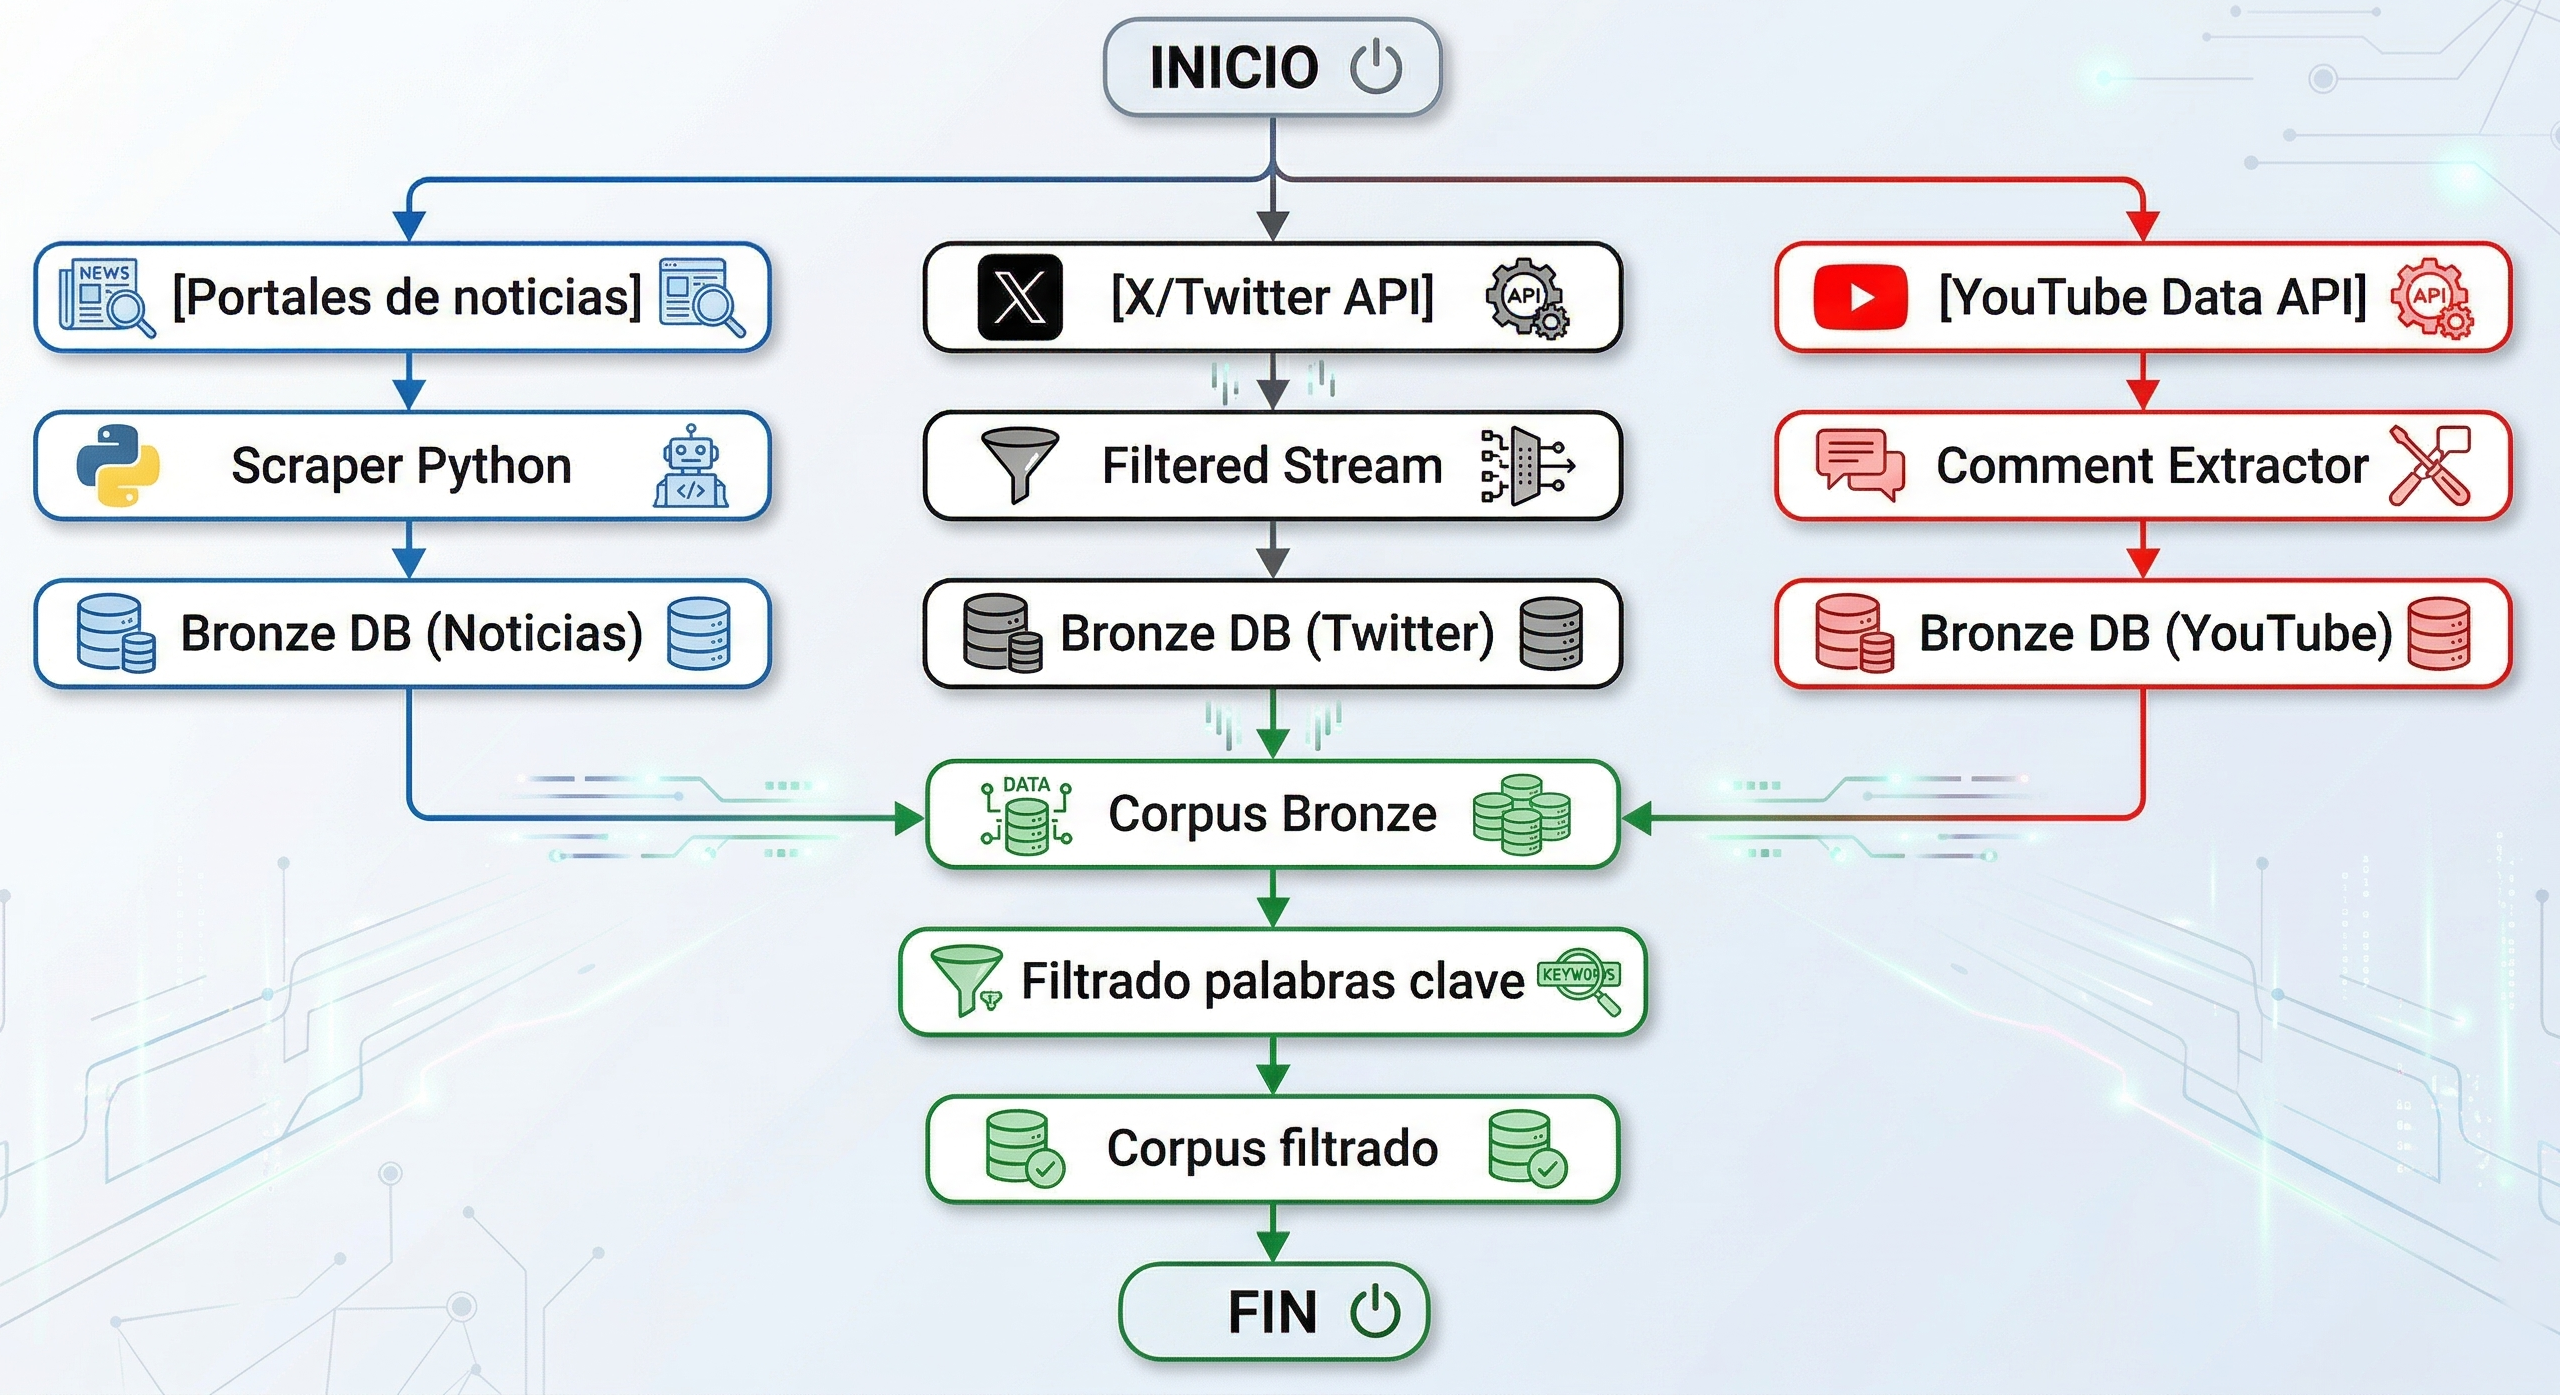
\includegraphics[width=0.90\textwidth]{3/figures/flujo_recoleccion.png}
        \caption[Flujograma de recolección de los conjuntos de datos del corpus electoral]{Flujograma de recolección de los conjuntos de datos del corpus electoral: noticias digitales, comentarios de YouTube y tweets de X/Twitter, con sus respectivos procesos de filtrado y almacenamiento en la capa Bronze de la arquitectura Medallion.\\
            Fuente: Elaboración propia.}
        \label{4:fig1}
    \end{center}
\end{figure}
 
Asimismo, para identificar y filtrar las publicaciones relevantes para el análisis, se
definió un diccionario de palabras clave y aliases electorales que incluye los nombres
completos, apodos, partidos y hashtags de los candidatos presidenciales en liza, así como
términos relacionados con los principales temas de la campaña: economía, seguridad,
educación, salud, corrupción y gobernabilidad.
 
\section{Técnicas para el procesamiento y análisis de la información}
 
\subsection{Metodología de implementación de la solución}
 
Como se explicó en el Capítulo II del presente trabajo, dentro de los sistemas de
analítica de negocio, Big Data y Minería de Datos, las tres metodologías más usadas son
CRISP-DM, SEMMA y KDD \parencite{tec_braulio2015metodologiasdm}. Para elegir la
metodología de implementación, se elaboró la Tabla \ref{4:table2} con el fin de comparar
las utilizadas por los autores en los antecedentes de esta investigación.
 
\vspace{2ex}
\begingroup
\renewcommand\arraystretch{0.3}
\begin{longtable}{M{3cm}M{2.5cm}M{2.5cm}M{6cm}}
    \caption[Cuadro comparativo para la selección de la metodología]{Cuadro comparativo para la selección de la metodología de implementación.}
    \label{4:table2}
    \footnotesize
    \centering
    \small
    \tabularnewline \specialrule{.1em}{.05em}{.05em}
    Metodología & Cantidad de referencias & Número de pasos & Nombre de los pasos \\
    \specialrule{.1em}{.05em}{.05em}
    {CRISP-DM}
    & 2
    & 6
    & \setlist{nolistsep}
    \begin{itemize}[label={--},nosep,noitemsep,leftmargin=*,topsep=0pt,partopsep=0pt]
        \item Comprensión del negocio.
        \item Comprensión de los datos.
        \item Preparación de los datos.
        \item Modelado.
        \item Evaluación.
        \item Despliegue.
    \end{itemize}
    \\
    \hline
    {Grupo A}
    & 2
    & 6
    & \setlist{nolistsep}
    \begin{itemize}[label={--},nosep,noitemsep,leftmargin=*,topsep=0pt,partopsep=0pt]
        \item Formulación del problema.
        \item Recolección de datos multicanal.
        \item Preprocesamiento de texto.
        \item Análisis con LLM.
        \item Evaluación.
        \item Despliegue.
    \end{itemize}
    \\
    \hline
    {Grupo B}
    & 2
    & 5
    & \setlist{nolistsep}
    \begin{itemize}[label={--},nosep,noitemsep,leftmargin=*,topsep=0pt,partopsep=0pt]
        \item Recolección de datos.
        \item Preprocesamiento y filtrado.
        \item Análisis de sentimientos.
        \item Detección de temas.
        \item Evaluación.
    \end{itemize}
    \\
    \hline
    {Grupo C}
    & 2
    & 5
    & \setlist{nolistsep}
    \begin{itemize}[label={--},nosep,noitemsep,leftmargin=*,topsep=0pt,partopsep=0pt]
        \item Formulación del problema.
        \item Recolección de datos.
        \item Preprocesamiento de datos.
        \item Modelado y análisis.
        \item Evaluación.
    \end{itemize}
    \\
    \hline
    {Grupo D}
    & 1
    & 4
    & \setlist{nolistsep}
    \begin{itemize}[label={--},nosep,noitemsep,leftmargin=*,topsep=0pt,partopsep=0pt]
        \item Recolección de datos.
        \item Preprocesamiento.
        \item Análisis LLM y clustering.
        \item Evaluación.
    \end{itemize}
    \\
    \specialrule{.1em}{.05em}{.05em}
\end{longtable}
\endgroup
\begin{flushleft}
    \small Fuente: Elaboración propia.
\end{flushleft}
 
De las tres metodologías mencionadas por \citeauthor{tec_braulio2015metodologiasdm},
la mayoría de los antecedentes revisados siguen secuencias de actividades comprendidas
dentro de CRISP-DM, incluyendo fases de comprensión del negocio, recolección y
preparación de datos, modelado y evaluación. Además, las siguientes características de la
literatura influyeron en la elección de la metodología CRISP-DM para el presente trabajo:
 
\begin{itemize}
    \item La metodología contempla entre sus fases la comprensión del negocio además
    de la parte técnica. Esta fase es crucial ya que en ella se define el problema a resolver
    —la falta de un sistema de análisis automatizado de percepción pública electoral en
    tiempo real— y se establecen los objetivos del sistema.
 
    \item Ayuda a los responsables del proyecto en la planificación y toma de decisiones
    (fase de Despliegue) a partir de los resultados obtenidos, convirtiendo los indicadores
    del sistema en oportunidades para mejorar la campaña de inteligencia electoral.
 
    \item Evalúa en todo el proceso los datos y configuraciones del modelo con el fin de
    construir el mejor pipeline. Estas evaluaciones son importantes para interpretar los
    resultados y tomar decisiones sobre la arquitectura del sistema.
 
    \item A diferencia de SEMMA, que comienza directamente con el muestreo sin hacer
    hincapié en la comprensión del contexto, y de KDD, cuyo enfoque es más técnico y
    orientado a métricas sin considerar el entorno del negocio, CRISP-DM contempla
    explícitamente la formulación del problema, presente en el actual trabajo.
\end{itemize}
 
Cada una de las fases de la metodología seleccionada, adaptada al contexto de la
inteligencia electoral con LLMs, se detalla en la Figura \ref{4:fig2}.
 
\begin{figure}[!ht]
    \begin{center}
        \includegraphics[width=1\textwidth]{3/figures/metodologia_crispdm.png}
        \caption[Metodología CRISP-DM adaptada al sistema de inteligencia electoral con LLMs]{Metodología CRISP-DM adaptada al sistema de inteligencia electoral con LLMs, mostrando las seis fases, su carácter iterativo y los entregables de cada etapa.\\
            Fuente: Elaboración propia.}
        \label{4:fig2}
    \end{center}
\end{figure}
 
Durante el proceso de implementación de la metodología, se definió construir un pipeline
de análisis multicanal que integra análisis de sentimientos con LLMs, detección dinámica
de temas con BERTopic y un grafo de conocimiento con Neo4j, arquitectura denominada
\textbf{GraphRAG Electoral}. De acuerdo a la literatura de los antecedentes revisados,
se analizaron las siguientes posibles fuentes de datos a incorporar:
 
\begin{itemize}
    \item \textbf{Noticias digitales}: \cite{pr_alvarez2023llm_political}, \cite{pr_mendonca2025bertopic_political}, \cite{pr_alvi2023twitter_election_review}.
    \item \textbf{Publicaciones en X/Twitter}: \cite{pr_gujral2024llm_elections}, \cite{pr_alvi2023twitter_election_review}, \cite{pr_mendonca2025bertopic_political}.
    \item \textbf{Comentarios de YouTube}: \cite{pr_chen2024combating_misinformation}.
    \item \textbf{Datos de encuestas electorales}: \cite{pr_gujral2024llm_elections}.
\end{itemize}
 
De las anteriores fuentes, los datos de encuestas electorales no fueron incluidos en el
pipeline principal de procesamiento ya que se utilizan exclusivamente como conjunto de
validación para calibrar los indicadores del sistema, y no como datos de entrada para el
análisis de sentimientos. Finalmente, fueron seleccionadas las tres fuentes principales
—noticias digitales, X/Twitter y comentarios de YouTube— cuya arquitectura de
recolección, procesamiento y análisis se detalla en las subsecciones siguientes.
 
El marco de trabajo del sistema propuesto, denominado \textbf{Pipeline GraphRAG
Electoral}, se estructura según la arquitectura Medallion en tres capas de datos
(Bronze, Silver y Gold) y cinco etapas de procesamiento, como se aprecia en la
Figura \ref{4:fig3}.
 
\begin{figure}[!ht]
    \begin{center}
        \includegraphics[width=0.92\textwidth]{3/figures/framework_graphrag.png}
        \caption[Marco de trabajo del Pipeline GraphRAG Electoral propuesto]{Marco de trabajo del Pipeline GraphRAG Electoral: arquitectura Medallion con tres capas de datos (Bronze, Silver, Gold) y cinco etapas de procesamiento desde la ingesta hasta la generación de indicadores de percepción pública.\\
            Fuente: Elaboración propia.}
        \label{4:fig3}
    \end{center}
\end{figure}
 
\subsubsection{Comprensión del negocio}
 
En la primera fase, se definió el problema a partir de comprender el contexto del proceso
electoral peruano y la necesidad de un sistema automatizado de inteligencia electoral. Las
actividades y tareas de esta fase se presentan en la Tabla \ref{4:table3}.
 
\vspace{2ex}
\begingroup
\renewcommand\arraystretch{0.3}
\begin{longtable}{m{5cm}m{5cm}M{5cm}}
    \caption[Actividades de la fase Comprensión del negocio]{Actividades de la fase Comprensión del negocio.}
    \label{4:table3}
    \footnotesize
    \small
    \tabularnewline \specialrule{.1em}{.05em}{.05em}
    \centering Actividades & \centering Descripción & Tareas \\
    \specialrule{.1em}{.05em}{.05em}
    Definir problema, objetivos e hipótesis.
    & Definición del problema central, los objetivos generales y específicos, y las hipótesis de investigación.
    & \setlist{nolistsep}
    \begin{itemize}[label={--},nosep,noitemsep,leftmargin=*,topsep=0pt,partopsep=0pt]
        \item Identificar la brecha en el análisis de percepción electoral digital.
        \item Definir los objetivos del sistema de inteligencia electoral.
        \item Formular las hipótesis del trabajo.
    \end{itemize}
    \\
    \hline
    Desarrollar la literatura de la investigación.
    & Revisión de antecedentes y trabajos previos sobre análisis de sentimientos político, LLMs y detección de temas.
    & \setlist{nolistsep}
    \begin{itemize}[label={--},nosep,noitemsep,leftmargin=*,topsep=0pt,partopsep=0pt]
        \item Buscar publicaciones académicas sobre LLMs en contextos electorales.
        \item Buscar material sobre BERTopic y GraphRAG aplicado a datos políticos.
    \end{itemize}
    \\
    \hline
    Definir metodología y arquitectura del sistema.
    & Selección de la metodología de implementación y diseño de la arquitectura del pipeline.
    & \setlist{nolistsep}
    \begin{itemize}[label={--},nosep,noitemsep,leftmargin=*,topsep=0pt,partopsep=0pt]
        \item Evaluar metodologías de la literatura.
        \item Seleccionar la metodología CRISP-DM.
        \item Diseñar la arquitectura Medallion del sistema.
    \end{itemize}
    \\
    \specialrule{.1em}{.05em}{.05em}
\end{longtable}
\endgroup
\begin{flushleft}
    \small Fuente: Elaboración propia.
\end{flushleft}
 
\textbf{Actividad 1: Definir problema, objetivos e hipótesis}
 
En esta actividad se detalla cómo se identificó la brecha existente en el análisis automatizado de la percepción pública electoral digital en el Perú, se formularon los objetivos de la investigación y se plantearon las hipótesis que guían el trabajo experimental.
 
\textbf{Entregable}: Problema, objetivos e hipótesis definidos.
 
\textbf{Actividad 2: Desarrollar la literatura de la investigación}
 
A partir de los objetivos definidos, se realizó la búsqueda de antecedentes académicos relacionados con el uso de LLMs en contextos electorales, minería de sentimientos político en español, detección dinámica de temas con BERTopic y sistemas GraphRAG. Se elaboró el marco teórico y conceptual descritos en el Capítulo II del presente trabajo.
 
\textbf{Entregable}: Marco teórico, antecedentes y conceptos operacionales de la investigación.
 
\textbf{Actividad 3: Definir metodología y arquitectura del sistema}
 
Luego de revisar los antecedentes y comparar las metodologías utilizadas por cada autor, se seleccionó CRISP-DM como metodología de implementación y se diseñó la arquitectura Medallion del pipeline GraphRAG Electoral.
 
\textbf{Entregable}: Metodología de implementación y arquitectura del sistema.
 
\subsubsection{Comprensión de los datos}
 
La segunda fase abarcó la recolección y el análisis estadístico exploratorio del corpus
electoral multicanal. Los datos utilizados comprenden publicaciones de tres fuentes
principales recolectadas durante el período de campaña presidencial. La lista de
actividades y tareas se presenta en la Tabla \ref{4:table4}.
 
\vspace{2ex}
\begingroup
\renewcommand\arraystretch{0.3}
\begin{longtable}{m{4cm}m{5.5cm}M{5.5cm}}
    \caption[Actividades de la fase Comprensión de los datos]{Actividades de la fase Comprensión de los datos.}
    \label{4:table4}
    \footnotesize
    \small
    \tabularnewline \specialrule{.1em}{.05em}{.05em}
    \centering Actividades & \centering Descripción & Tareas \\
    \specialrule{.1em}{.05em}{.05em}
    Construir corpus de noticias digitales.
    & Construcción del corpus de artículos y titulares de los principales portales de prensa peruanos (capa Bronze).
    & \setlist{nolistsep}
    \begin{itemize}[label={--},nosep,noitemsep,leftmargin=*,topsep=0pt,partopsep=0pt]
        \item Diseñar scrapers para portales de noticias objetivo.
        \item Recolectar artículos con URL, fecha, titular y texto.
        \item Almacenar datos crudos en capa Bronze.
    \end{itemize}
    \\
    \hline
    Construir corpus de X/Twitter.
    & Construcción del corpus de tweets relacionados con los candidatos presidenciales mediante la API de X.
    & \setlist{nolistsep}
    \begin{itemize}[label={--},nosep,noitemsep,leftmargin=*,topsep=0pt,partopsep=0pt]
        \item Configurar conexión con la API Filtered Stream de X.
        \item Definir palabras clave, hashtags y cuentas de interés.
        \item Almacenar tweets con metadatos en capa Bronze.
    \end{itemize}
    \\
    \hline
    Construir corpus de YouTube.
    & Construcción del corpus de comentarios de usuarios en videos electorales de YouTube.
    & \setlist{nolistsep}
    \begin{itemize}[label={--},nosep,noitemsep,leftmargin=*,topsep=0pt,partopsep=0pt]
        \item Identificar videos electorales mediante YouTube Data API.
        \item Recolectar comentarios con ID de usuario y fecha.
        \item Almacenar comentarios crudos en capa Bronze.
    \end{itemize}
    \\
    \hline
    Realizar análisis exploratorio del corpus.
    & Análisis estadístico y exploratorio de las variables del corpus para cada fuente de datos.
    & \setlist{nolistsep}
    \begin{itemize}[label={--},nosep,noitemsep,leftmargin=*,topsep=0pt,partopsep=0pt]
        \item Describir distribución temporal y por fuente.
        \item Analizar longitud de textos y vocabulario.
        \item Identificar candidatos más mencionados.
    \end{itemize}
    \\
    \specialrule{.1em}{.05em}{.05em}
\end{longtable}
\endgroup
\begin{flushleft}
    \small Fuente: Elaboración propia.
\end{flushleft}
 
\textbf{Actividad 1: Construir corpus de noticias digitales}
 
De acuerdo a la Figura \ref{4:fig1}, en esta actividad se construyó el corpus de artículos de noticias digitales mediante scrapers diseñados en Python para los portales de prensa peruanos seleccionados. El proceso de recolección siguió el flujo de la Figura \ref{4:fig4}.
 
\begin{figure}[!ht]
    \begin{center}
        \includegraphics[width=0.80\textwidth]{3/figures/flujo_scraping_noticias.png}
        \caption[Proceso de recolección del corpus de noticias digitales]{Proceso de recolección del corpus de noticias digitales: desde la identificación de portales objetivo hasta el almacenamiento en la capa Bronze de la arquitectura Medallion.\\
            Fuente: Elaboración propia.}
        \label{4:fig4}
    \end{center}
\end{figure}
 
\textbf{Entregable}: Corpus de noticias digitales con URL, fecha, portal de origen, titular y texto completo del artículo.
 
\textbf{Actividad 2: Construir corpus de X/Twitter}
 
Una vez configurada la conexión con la API Filtered Stream de X, se definió el conjunto de palabras clave, hashtags y cuentas de candidatos que activan la captura en tiempo real. El proceso de recolección se realizó según el flujo de la Figura \ref{4:fig5}.
 
\begin{figure}[!ht]
    \begin{center}
        \includegraphics[width=0.80\textwidth]{3/figures/flujo_api_twitter.png}
        \caption[Proceso de recolección del corpus de X/Twitter mediante API Filtered Stream]{Proceso de recolección del corpus de X/Twitter: configuración de reglas de filtrado, captura en streaming y almacenamiento con metadatos en capa Bronze.\\
            Fuente: Elaboración propia.}
        \label{4:fig5}
    \end{center}
\end{figure}
 
\textbf{Entregable}: Corpus de tweets con ID, texto, fecha, número de retweets y menciones a candidatos.
 
\textbf{Actividad 3: Construir corpus de YouTube}
 
Mediante la YouTube Data API, se identificaron los videos electorales más relevantes y se recolectaron sus comentarios de usuarios, excluyendo los publicados por los propios canales de los candidatos para evitar sesgo en la muestra ciudadana. El proceso se detalla en la Figura \ref{4:fig6}.
 
\begin{figure}[!ht]
    \begin{center}
        \includegraphics[width=0.80\textwidth]{3/figures/flujo_youtube_comentarios.png}
        \caption[Proceso de recolección del corpus de comentarios de YouTube]{Proceso de extracción de comentarios de usuarios en videos electorales de YouTube, desde la identificación de videos relevantes hasta el almacenamiento en capa Bronze.\\
            Fuente: Elaboración propia.}
        \label{4:fig6}
    \end{center}
\end{figure}
 
\textbf{Entregable}: Corpus de comentarios de YouTube con ID de video, texto del comentario, fecha y número de likes.
 
\textbf{Actividad 4: Realizar análisis exploratorio del corpus}
 
En esta actividad se realizó el análisis estadístico descriptivo de los tres corpus recolectados: distribución temporal de publicaciones, longitud promedio de textos, distribución de menciones por candidato y por fuente, y análisis del vocabulario electoral dominante mediante nubes de palabras.
 
\textbf{Entregable}: Gráficos estadísticos y descriptivos del corpus por fuente de datos.
 
\subsubsection{Preparación de los datos}
 
En la tercera fase, los datos crudos de la capa Bronze se transformaron en la capa Silver
mediante un conjunto de procesos de limpieza, normalización y enriquecimiento. Las
actividades de esta etapa se detallan en la Tabla \ref{4:table5}.
 
\vspace{2ex}
\begingroup
\renewcommand\arraystretch{0.3}
\begin{longtable}{m{5cm}m{5cm}M{5cm}}
    \caption[Actividades de la fase Preparación de los datos]{Actividades de la fase Preparación de los datos.}
    \label{4:table5}
    \footnotesize
    \small
    \tabularnewline \specialrule{.1em}{.05em}{.05em}
    \centering Actividades & \centering Descripción & Tareas \\
    \specialrule{.1em}{.05em}{.05em}
    Limpiar y normalizar el corpus.
    & Preprocesamiento textual de las publicaciones de las tres fuentes para su análisis con LLM.
    & \setlist{nolistsep}
    \begin{itemize}[label={--},nosep,noitemsep,leftmargin=*,topsep=0pt,partopsep=0pt]
        \item Eliminar spam, bots y publicaciones duplicadas.
        \item Normalizar caracteres especiales, emojis y URLs.
        \item Detectar y filtrar publicaciones en idiomas distintos al español.
    \end{itemize}
    \\
    \hline
    Segmentar el corpus para análisis.
    & División de textos largos en segmentos procesables por el LLM respetando la ventana de contexto.
    & \setlist{nolistsep}
    \begin{itemize}[label={--},nosep,noitemsep,leftmargin=*,topsep=0pt,partopsep=0pt]
        \item Definir tamaño máximo de segmento en tokens.
        \item Implementar segmentación con superposición de contexto.
        \item Registrar relación documento-segmento en base de datos.
    \end{itemize}
    \\
    \hline
    Construir diccionario de aliases electorales.
    & Creación del diccionario de names, apodos y aliases de candidatos para el filtrado con Aho-Corasick.
    & \setlist{nolistsep}
    \begin{itemize}[label={--},nosep,noitemsep,leftmargin=*,topsep=0pt,partopsep=0pt]
        \item Recopilar nombres completos y apodos de candidatos.
        \item Incluir nombres de partidos y lemas de campaña.
        \item Construir el autómata Aho-Corasick para búsqueda eficiente.
    \end{itemize}
    \\
    \specialrule{.1em}{.05em}{.05em}
\end{longtable}
\endgroup
\begin{flushleft}
    \small Fuente: Elaboración propia.
\end{flushleft}
 
\textbf{Actividad 1: Limpiar y normalizar el corpus}
 
En esta actividad se aplicó un pipeline de preprocesamiento textual sobre los tres corpus de la capa Bronze. El proceso incluyó la eliminación de spam y cuentas de bots identificadas mediante patrones de comportamiento, la normalización de emojis (convertidos a texto descriptivo), la eliminación de URLs y menciones de usuario, y la detección automática de idioma mediante la librería \texttt{langdetect} para conservar únicamente publicaciones en español.
 
\textbf{Entregable}: Corpus limpio y normalizado, listo para análisis con LLM.
 
\textbf{Actividad 2: Segmentar el corpus para análisis}
 
Dado que los artículos de noticias superan en longitud la ventana de contexto del LLM utilizado, se implementó un proceso de segmentación con superposición que divide cada documento en segmentos de máximo 512 tokens con una superposición de 50 tokens entre segmentos consecutivos, preservando el contexto necesario para el análisis de sentimientos a nivel de aspecto.
 
\textbf{Entregable}: Tabla de segmentos con relación uno-a-muchos hacia la tabla de documentos originales (capa Silver).
 
\textbf{Actividad 3: Construir diccionario de aliases electorales}
 
Se construyó el diccionario de aliases que alimenta el autómata Aho-Corasick descrito en el pipeline. Este diccionario incluye los nombres completos, apodos, partidos políticos y lemas de campaña de todos los candidatos presidenciales, permitiendo detectar menciones implícitas y coloquiales que un buscador de texto exacto no capturaría. Este paso es fundamental para garantizar que el LLM solo analice segmentos que efectivamente contienen referencias a candidatos, reduciendo el costo computacional en un factor proporcional al número de aliases registrados.
 
\textbf{Entregable}: Diccionario de aliases y autómata Aho-Corasick compilado.
 
\subsubsection{Modelamiento}
 
Al concluir la preparación de los datos, los segmentos del corpus enriquecido fueron
procesados por el pipeline de análisis con LLMs. Las actividades de esta fase se detallan
en la Tabla \ref{4:table6}.
 
\vspace{2ex}
\begingroup
\renewcommand\arraystretch{0.3}
\begin{longtable}{m{4.6cm}m{4.9cm}M{5.5cm}}
    \caption[Actividades de la fase Modelamiento]{Actividades de la fase Modelamiento.}
    \label{4:table6}
    \footnotesize
    \small
    \tabularnewline \specialrule{.1em}{.05em}{.05em}
    \centering Actividades & \centering Descripción & Tareas \\
    \specialrule{.1em}{.05em}{.05em}
    Desarrollar módulo de análisis de sentimientos con LLM.
    & Implementación del análisis de sentimientos a nivel de aspecto mediante prompts diseñados para el contexto electoral peruano.
    & \setlist{nolistsep}
    \begin{itemize}[label={--},nosep,noitemsep,leftmargin=*,topsep=0pt,partopsep=0pt]
        \item Diseñar prompt de análisis con estructura role-context-task-format.
        \item Implementar llamadas a la API del LLM con respuesta JSON estructurada.
        \item Validar outputs y gestionar errores de parsing.
    \end{itemize}
    \\
    \hline
    Desarrollar módulo de detección dinámica de temas.
    & Implementación del pipeline BERTopic para clustering semántico de temas electorales.
    & \setlist{nolistsep}
    \begin{itemize}[label={--},nosep,noitemsep,leftmargin=*,topsep=0pt,partopsep=0pt]
        \item Generar embeddings con Sentence-BERT multilingüe.
        \item Reducir dimensionalidad con UMAP.
        \item Aplicar HDBSCAN para clustering inductivo.
        \item Etiquetar clusters con LLM mediante c-TF-IDF.
    \end{itemize}
    \\
    \hline
    Construir grafo de conocimiento electoral.
    & Implementación del grafo Neo4j con nodos y relaciones del ecosistema electoral digital.
    & \setlist{nolistsep}
    \begin{itemize}[label={--},nosep,noitemsep,leftmargin=*,topsep=0pt,partopsep=0pt]
        \item Definir esquema de nodos (Candidato, Tema, Fuente, Periodo, Evento).
        \item Implementar jobs de agregación semanal con MERGE idempotente.
        \item Calcular relaciones MENCIONA, CO\_OCURRE, CUBRE y REACCIONA\_A.
    \end{itemize}
    \\
    \hline
    Implementar sistema GraphRAG para consultas.
    & Desarrollo del módulo de consulta en lenguaje natural sobre el grafo de conocimiento electoral.
    & \setlist{nolistsep}
    \begin{itemize}[label={--},nosep,noitemsep,leftmargin=*,topsep=0pt,partopsep=0pt]
        \item Inyectar schema del grafo al contexto del LLM.
        \item Implementar traducción de preguntas en español a consultas Cypher.
        \item Validar respuestas con evidencia textual de los documentos originales.
    \end{itemize}
    \\
    \specialrule{.1em}{.05em}{.05em}
\end{longtable}
\endgroup
\begin{flushleft}
    \small Fuente: Elaboración propia.
\end{flushleft}
 
\textbf{Actividad 1: Desarrollar módulo de análisis de sentimientos con LLM}
 
En esta actividad se diseñó el prompt de análisis de sentimientos a nivel de aspecto y se
implementó el módulo de llamadas a la API del LLM. El prompt sigue la estructura de
cinco componentes (rol, contexto, instrucción, formato y ejemplos few-shot) descrita en el
marco conceptual, y extrae en una sola llamada por segmento: candidatos detectados,
método de detección, nivel de confianza, score de sentimiento en escala $[-1, 1]$,
fragmento clave que justifica el sentimiento, temas identificados y relaciones entre temas.
Para la selección del LLM, se realizó un benchmarking sobre las propuestas de los
autores de los antecedentes:
 
\begin{itemize}
    \item \textbf{Gemini (Google)}: \cite{pr_alvarez2023llm_political}, arquitectura del HTML de metodología adjunto.
    \item \textbf{GPT-4 (OpenAI)}: \cite{pr_gujral2024llm_elections}, \cite{pr_chen2024combating_misinformation}.
    \item \textbf{Llama 2 (Meta, código abierto)}: \cite{pr_gujral2024llm_elections}.
    \item \textbf{mBERT / XLM-RoBERTa (modelos encoder)}: \cite{pr_alvi2023twitter_election_review}.
\end{itemize}
 
De acuerdo a los resultados de los antecedentes, los modelos generativos (GPT-4, Gemini)
superan a los modelos encoder en precisión contextual para análisis de sentimientos
político en español, especialmente en el manejo de ironía, sarcasmo y ambigüedad
semántica. Dado que la investigación requiere análisis en tiempo real con respuestas JSON
estructuradas, se seleccionó la API de Gemini Flash como modelo principal por su relación
entre capacidad y latencia, y GPT-4o como modelo de validación para los experimentos de
evaluación.
 
\textbf{Entregable}: Módulo de análisis de sentimientos con LLM y tabla \texttt{analisis} de la capa Silver.
 
\textbf{Actividad 2: Desarrollar módulo de detección dinámica de temas}
 
En esta actividad se implementó el pipeline BERTopic para la detección dinámica de temas.
Se generaron embeddings de oraciones mediante el modelo paraphrase-multilingual-MiniLM-L12-v2
de Sentence-BERT, optimizado para español. Para el clustering, se utilizó HDBSCAN
inductivo con \texttt{min\_cluster\_size=10} y \texttt{min\_samples=3}, parámetros que
permiten detectar temas con al menos 10 publicaciones asociadas sin requerir definir el
número de temas a priori. Gemini etiqueta cada cluster resultante en una sola llamada
por cluster, procesando los 15 términos más representativos de cada grupo según c-TF-IDF.
La elección de HDBSCAN sobre K-Means se justifica en que, a diferencia de este último, no
requiere especificar el número de clusters y descarta automáticamente publicaciones ruidosas
que no pertenecen a ningún tema coherente, siguiendo el enfoque de
\cite{pr_mendonca2025bertopic_political} y \cite{pr_janssens2025bertopic_llm}.
 
\textbf{Entregable}: Pipeline BERTopic configurado y taxonomía de temas electorales generada.
 
\textbf{Actividad 3: Construir grafo de conocimiento electoral}
 
En esta actividad se implementó el grafo de conocimiento electoral en Neo4j, con el
esquema de cinco tipos de nodos (Candidato, Tema, Fuente, Evento y Periodo) y ocho
tipos de relaciones (MENCIONA, MENCIONA\_CIUDADANO, EN\_PERIODO, CO\_OCURRE, CUBRE,
SILENCIA, REACCIONA\_A y OCURRE\_EN) con su respectiva metadata de aristas, como se
describe en el marco de la metodología GraphRAG. Los jobs de agregación semanal utilizan
la cláusula \texttt{MERGE} de Cypher para que el proceso sea idempotente: si ya existe
la arista para una semana, actualiza sus valores; si no existe, la crea. Esta propiedad
garantiza que el grafo pueda repoblarse sin duplicar datos.
 
\textbf{Entregable}: Grafo de conocimiento electoral en Neo4j con datos agregados semanalmente.
 
\textbf{Actividad 4: Implementar sistema GraphRAG para consultas}
 
En esta actividad se implementó el módulo de consulta en lenguaje natural sobre el grafo
electoral. El sistema inyecta el schema completo del grafo al contexto del LLM en cada
consulta, junto con ejemplos de preguntas-Cypher en modalidad few-shot, lo que permite
al modelo traducir preguntas en español como «¿Qué temas co-ocurren con corrupción
en cobertura negativa?» a consultas Cypher válidas sobre el grafo de Neo4j. Las respuestas
son fundamentadas con fragmentos textuales de los documentos originales, garantizando
la trazabilidad de cada hallazgo hasta su fuente primaria.
 
\textbf{Entregable}: Módulo GraphRAG funcional con ejemplos de consultas en lenguaje natural validados.
 
\subsubsection{Evaluación}
 
Esta fase comprende la evaluación del sistema de inteligencia electoral a través de las
métricas de clasificación y calidad de temas seleccionadas. Las actividades y tareas
seguidas se detallan en la Tabla \ref{4:table7}.
 
\begin{longtable}{m{5cm}m{4.5cm}M{5.5cm}}
    \caption[Actividades de la fase Evaluación]{Actividades de la fase Evaluación.}
    \label{4:table7}
    \footnotesize
    \small
    \tabularnewline \specialrule{.1em}{.05em}{.05em}
    \centering Actividades & \centering Descripción & Tareas \\
    \specialrule{.1em}{.05em}{.05em}
    Evaluar módulo de análisis de sentimientos.
    & Evaluación del desempeño del análisis de sentimientos comparando los resultados del LLM con etiquetas humanas de referencia.
    & \setlist{nolistsep}
    \begin{itemize}[label={--},nosep,noitemsep,leftmargin=*,topsep=0pt,partopsep=0pt]
        \item Construir conjunto de validación con etiquetas humanas.
        \item Calcular exactitud, precisión, sensibilidad y F1.
        \item Comparar resultados entre distintas configuraciones de prompt.
    \end{itemize}
    \\
    \hline
    Evaluar módulo de detección de temas.
    & Evaluación de la coherencia semántica y diversidad de los temas detectados por BERTopic.
    & \setlist{nolistsep}
    \begin{itemize}[label={--},nosep,noitemsep,leftmargin=*,topsep=0pt,partopsep=0pt]
        \item Calcular coherencia C\textsubscript{v} de los temas.
        \item Evaluar diversidad temática del corpus.
        \item Validar etiquetas de clusters con analistas políticos.
    \end{itemize}
    \\
    \hline
    Evaluar sistema GraphRAG.
    & Evaluación de la precisión de las consultas Cypher generadas y la calidad de las respuestas en lenguaje natural.
    & \setlist{nolistsep}
    \begin{itemize}[label={--},nosep,noitemsep,leftmargin=*,topsep=0pt,partopsep=0pt]
        \item Diseñar conjunto de preguntas de evaluación con respuesta esperada.
        \item Medir exactitud de las consultas Cypher generadas.
        \item Evaluar factualidad y trazabilidad de las respuestas.
    \end{itemize}
    \\
    \hline
    Evaluar el sistema integrado.
    & Evaluación del pipeline completo en términos de latencia, escalabilidad y correlación con encuestas de opinión.
    & \setlist{nolistsep}
    \begin{itemize}[label={--},nosep,noitemsep,leftmargin=*,topsep=0pt,partopsep=0pt]
        \item Medir latencia extremo a extremo del pipeline.
        \item Comparar indicadores ISN con encuestas electorales disponibles.
        \item Evaluar correlación de Pearson entre ambas fuentes.
    \end{itemize}
    \\
    \specialrule{.1em}{.05em}{.05em}
\end{longtable}
\begin{flushleft}
    \small Fuente: Elaboración propia.
\end{flushleft}
 
\subsubsection{Despliegue}
 
En la última fase de la metodología, el sistema de inteligencia electoral fue desplegado
como un prototipo funcional accesible para analistas políticos y periodistas. Las
actividades de esta fase se detallan en la Tabla \ref{4:table8}.
 
\begin{longtable}{m{4.5cm}m{5.3cm}M{5.2cm}}
    \caption[Actividades de la fase Despliegue]{Actividades de la fase Despliegue.}
    \label{4:table8}
    \footnotesize
    \centering
    \small
    \tabularnewline \specialrule{.1em}{.05em}{.05em}
    \centering Actividades & \centering Descripción & Tareas \\
    \specialrule{.1em}{.05em}{.05em}
    Diseñar dashboard de visualización.
    & Diseño e implementación del dashboard interactivo que muestra los indicadores de percepción pública en tiempo real.
    & \setlist{nolistsep}
    \begin{itemize}[label={--},nosep,noitemsep,leftmargin=*,topsep=0pt,partopsep=0pt]
        \item Diseñar vistas para ISN, IRT e IVE por candidato y período.
        \item Implementar gráficos de evolución temporal y mapas de calor temáticos.
        \item Integrar módulo de consulta GraphRAG en lenguaje natural.
    \end{itemize}
    \\
    \hline
    Ejecutar prototipo con datos electorales en vivo.
    & Ejecución del sistema completo en condiciones reales durante el período de campaña presidencial.
    & \setlist{nolistsep}
    \begin{itemize}[label={--},nosep,noitemsep,leftmargin=*,topsep=0pt,partopsep=0pt]
        \item Activar pipeline de ingesta en tiempo real.
        \item Monitorear indicadores y detectar anomalías.
        \item Generar reportes automáticos diarios.
    \end{itemize}
    \\
    \specialrule{.1em}{.05em}{.05em}
\end{longtable}
\begin{flushleft}
    \small Fuente: Elaboración propia.
\end{flushleft}
 
Luego de evaluar el desempeño de cada módulo del sistema, se compararon los resultados
con los antecedentes revisados y se desarrolló una prueba piloto en la que el sistema
completo fue ejecutado en tiempo real durante una semana de campaña electoral. Los
detalles de esta prueba y sus resultados se presentan en el Capítulo V.
 
\subsection{Metodología para la medición de resultados}
 
Para evaluar la performance de los módulos del sistema, que corresponde a la quinta fase
de la metodología CRISP-DM, se utilizaron diversas métricas como instrumentos de
medición de desempeño. A continuación, se detallan su concepto y fórmulas de cálculo.
 
\begin{itemize}
    \item \textbf{Matriz de confusión}: Es una tabla de $N \times N$ que resume el nivel de
    éxito de las predicciones de un modelo de clasificación. Para el módulo de análisis de
    sentimientos, $N=3$ (positivo, negativo, neutral), permitiendo identificar los errores más
    frecuentes de clasificación (por ejemplo, confundir sentimiento neutro con negativo en
    textos irónicos) \parencite{gl_kohavi1998ml_glossary}.
 
    \item \textbf{Exactitud} (\textit{accuracy}): Fracción de predicciones de sentimiento
    realizadas correctamente sobre el total de publicaciones en el conjunto de validación.
    Se calcula mediante la Ecuación \ref{eq:accuracy_llm}:
 
    \begin{equation}\label{eq:accuracy_llm}
    \phantomsection
    Exactitud = \frac{V.P. + V.N.}{V.P. + V.N. + F.P. + F.N.}
    \end{equation}
    \myequations{Fórmula para calcular la exactitud del módulo de sentimientos}
 
    \item \textbf{Precisión} (\textit{precision}): Proporción de publicaciones clasificadas
    correctamente como de sentimiento positivo sobre el total de publicaciones clasificadas
    como positivas por el sistema. Se calcula mediante la Ecuación \ref{eq:precision_llm}:
 
    \begin{equation}\label{eq:precision_llm}
    \phantomsection
    Precisi\acute{o}n = \frac{V.P.}{V.P. + F.P.}
    \end{equation}
    \myequations{Fórmula para calcular la precisión del módulo de sentimientos}
 
    \item \textbf{Sensibilidad} (\textit{recall}): Proporción de publicaciones realmente
    positivas que el sistema identifica correctamente. Se calcula mediante la Ecuación
    \ref{eq:recall_llm}:
 
    \begin{equation}\label{eq:recall_llm}
    \phantomsection
    Sensibilidad = \frac{V.P.}{V.P. + F.N.}
    \end{equation}
    \myequations{Fórmula para calcular la sensibilidad del módulo de sentimientos}
 
    \item \textbf{Puntaje F1}: Media armónica de la precisión y la sensibilidad. Se usa
    cuando las clases de sentimiento están desbalanceadas —lo que es frecuente en corpora
    electorales donde el sentimiento negativo predomina sobre el positivo— y no es posible
    dar una conclusión basada solo en exactitud. Se calcula mediante la Ecuación
    \ref{eq:f1_llm}:
 
    \begin{equation}\label{eq:f1_llm}
    \phantomsection
    Puntaje\ F1 = \frac{2 \times Precisi\acute{o}n \times Sensibilidad}{Precisi\acute{o}n + Sensibilidad}
    \end{equation}
    \myequations{Fórmula para calcular el puntaje F1 del módulo de sentimientos}
 
    \item \textbf{Coherencia semántica $C_v$}: Métrica estándar para evaluar la calidad de
    los temas generados por modelos de topic modeling. Mide la co-ocurrencia normalizada
    de los términos más representativos de cada tema en el corpus. Un valor de $C_v$
    cercano a 1 indica temas semánticamente coherentes. Se calcula mediante la Ecuación
    \ref{eq:cv_coherence}:
 
    \begin{equation}\label{eq:cv_coherence}
    \phantomsection
    C_v(t) = \frac{1}{\binom{|W|}{2}} \sum_{i>j} \log \frac{P(w_i, w_j) + \epsilon}{P(w_i) \cdot P(w_j)}
    \end{equation}
    \myequations{Fórmula para calcular la coherencia semántica $C_v$ de los temas detectados}
 
    Donde $W$ es el conjunto de los términos más representativos del tema $t$, $P(w_i, w_j)$
    es la probabilidad de co-ocurrencia de los términos $w_i$ y $w_j$ en el corpus, y
    $\epsilon$ es un suavizador para evitar logaritmos de cero.
 
    \item \textbf{Correlación de Pearson con encuestas}: Mide el grado de correlación
    lineal entre el Índice de Sentimiento Neto (ISN) calculado por el sistema para cada
    candidato y los resultados de las encuestas de intención de voto disponibles para el
    mismo período. Un coeficiente de Pearson alto ($r > 0.7$) indicaría que el sistema
    captura adecuadamente la percepción electoral real.
\end{itemize}
 
La elección de las anteriores métricas para evaluar cada módulo del sistema se realizó
luego de comparar las utilizadas por los autores en los antecedentes de la investigación:
 
\begin{itemize}
    \item \textbf{Exactitud}: \cite{pr_alvi2023twitter_election_review}, \cite{pr_gujral2024llm_elections}.
    \item \textbf{Precisión y Sensibilidad}: \cite{pr_alvarez2023llm_political}, \cite{pr_alvi2023twitter_election_review}.
    \item \textbf{Puntaje F1}: \cite{pr_alvarez2023llm_political}, \cite{pr_chen2024combating_misinformation}.
    \item \textbf{Coherencia semántica $C_v$}: \cite{pr_mendonca2025bertopic_political}, \cite{pr_janssens2025bertopic_llm}.
    \item \textbf{Correlación con encuestas}: \cite{pr_gujral2024llm_elections}.
\end{itemize}
 
\begin{landscape}
\section{Cronograma de actividades y presupuesto}
 
Se elaboró el cronograma de actividades de toda la investigación, mostrado en la
Figura \ref{4:fig7}, contemplando desde el inicio de la misma hasta la sustentación del
trabajo.
 
\begin{figure}[!ht]
    \begin{center}
        \includegraphics[width=1\textwidth]{3/figures/cronograma.png}
        \caption[Cronograma de actividades de la investigación]{Cronograma de actividades de la investigación, organizado por fases de la metodología CRISP-DM y distribuido en los meses del período de ejecución.\\
            Fuente: Elaboración propia.}
        \label{4:fig7}
    \end{center}
\end{figure}
\end{landscape}
 
Los costos personales del autor de la investigación se presentan en la Tabla
\ref{4:table9}.
 
\begin{table}[h!]
    \caption[Presupuesto de costos personales del autor]{Presupuesto de los costos personales del autor de la investigación.}
    \label{4:table9}
    \centering
    \small
    \begin{tabular}{lcrr}
        \specialrule{.1em}{.05em}{.05em}
        \multicolumn{1}{c}{Item} & \multicolumn{1}{c}{Tiempo (horas)} & \multicolumn{1}{c}{Costo (soles)} & \multicolumn{1}{c}{Subtotal} \\
        \specialrule{.1em}{.05em}{.05em}
        \multicolumn{4}{l}{Recursos materiales} \\
        Laptop para desarrollo (GPU integrada)        &        & S/.4,800.00  & S/.4,800.00  \\
        \hline
        \multicolumn{4}{l}{Trámites académicos} \\
        Inscripción a cursos de actualización y TSP         &        & S/.8500.00    & S/.8500.00    \\
        \hline
        \multicolumn{4}{l}{Recursos humanos} \\
        Avance de tesis                               & 900    & Incalculable & --           \\
        \hline
        \multicolumn{4}{l}{Servicios generales} \\
        Internet + electricidad (5 meses)             & 120    & S/.85.00     & S/.680.00    \\
        \specialrule{.1em}{.05em}{.05em}
        Total & & & S/.14,880.00 \\
        \specialrule{.1em}{.05em}{.05em}
    \end{tabular}
    \begin{flushleft}
        \small Fuente: Elaboración propia.
    \end{flushleft}
\end{table}
 
Los costos por uso de servicios en la nube necesarios para el procesamiento del corpus y
el entrenamiento de los modelos se presentan en la Tabla \ref{4:table10}.
 
\begin{table}[h!]
    \caption[Presupuesto de herramientas y servicios en la nube]{Presupuesto de los costos de herramientas y servicios en la nube utilizados en el proyecto.}
    \label{4:table10}
    \centering
    \small
    \begin{tabular}{lcrcr}
        \specialrule{.1em}{.05em}{.05em}
        \multicolumn{1}{c}{Item} & \multicolumn{1}{c}{Unidades} & \multicolumn{1}{c}{Costo (USD)} & \multicolumn{1}{c}{Horas} & \multicolumn{1}{c}{Subtotal} \\
        \specialrule{.1em}{.05em}{.05em}
        \multicolumn{4}{l}{Google Cloud Platform (GCP)} & -- \\
        Instancia VM para scraping (e2-medium, 4 GB RAM)  & 1  & \$0.034  & 400  & \$13.60  \\
        Cloud Run para pipeline en tiempo real             & 1  & \$0.024  & 300  & \$7.20   \\
        Cloud Storage para capa Bronze                     & 1  & \$0.020  & --   & \$8.00   \\
        BigQuery para capa Silver/Gold                     & 1  & \$5.00   & --   & \$15.00  \\
        \hline
        \multicolumn{4}{l}{API LLM} & -- \\
        Gemini Flash API (tokens de análisis)              & -- & \$0.075/1M & -- & \$45.00  \\
        OpenAI GPT-4o API (validación)                     & -- & \$5.00/1M  & -- & \$25.00  \\
        \hline
        \multicolumn{4}{l}{Neo4j AuraDB (grafo)} & -- \\
        Plan Professional (1 instancia)                    & 3  & \$65.00  & --   & \$195.00 \\
        \hline
        \multicolumn{4}{l}{X/Twitter API} & -- \\
        Plan Basic (hasta 10k tweets/mes)                  & 6  & \$100.00 & --   & \$600.00 \\
        \hline
        \multicolumn{4}{l}{YouTube Data API} & -- \\
        Cuota gratuita (10,000 unidades/día)               & -- & \$0.00   & --   & \$0.00   \\
        \specialrule{.1em}{.05em}{.05em}
        Total & & & & \$908.80 \\
        \specialrule{.1em}{.05em}{.05em}
    \end{tabular}
    \begin{flushleft}
        \small Fuente: Elaboración propia.
    \end{flushleft}
\end{table}